\documentclass[11pt]{article}

\usepackage[preprint]{acl}
\usepackage{times}
\usepackage{latexsym}
\usepackage[T1]{fontenc}
\usepackage[utf8]{inputenc}
\usepackage{microtype}
\usepackage{graphicx}
\usepackage{booktabs}
\usepackage{xcolor}
\usepackage{tikz}
\usetikzlibrary{arrows.meta}
\makeatletter
\g@addto@macro{\UrlBreaks}{\do\-}
\makeatother

% Red markers for anything that still needs a real number or a sentence from you.
% Search the PDF/TeX for "FILL" and "[?]" before submitting: none may remain.
\newcommand{\fillme}[1]{\textbf{\textcolor{red}{[FILL: #1]}}}
\newcommand{\ph}{\textbf{\textcolor{red}{[?]}}}

\title{Reproducing Sentence-BERT and Testing Its Generalisation \\ to Data-Engineering Text}

\author{
  Lokapal Haachagowdanahalli Shankarappa \\
  Master of Data Science, Macquarie University \\
  COMP8240: Applications of Data Science \\
  \texttt{lokapal.haachagowdanahallishankarappa@students.mq.edu.au} \\
}

\begin{document}
\maketitle

\begin{abstract}
This report describes a reproduction of Sentence-BERT (SBERT; \citealp{reimers2019sentence}), which fine-tunes BERT in a siamese network so that sentence embeddings can be compared with cosine similarity. I re-ran the paper's STS Benchmark evaluation using checkpoints released for the paper and a later model, then tested generalisation on an existing biomedical dataset and on a new 40-pair dataset of data-engineering questions that was scored by two human annotators and an LLM judge. The paper's own checkpoints reproduce its STS Benchmark scores to within 0.3 points, but on both new datasets the NLI-only checkpoint falls by 18 to 25 points, while a later model stays at about 81 to 84. I also discuss the limits of the evidence: the new dataset is small, its sentences were drafted with LLM assistance, and its design makes ranking easier than on natural data.
\end{abstract}

\section{The Paper and Why It Was Chosen}
\label{sec:paper}

\paragraph{What the paper does.}
Semantic textual similarity (STS) asks how close in meaning two sentences are. BERT \citep{devlin2019bert} processes both sentences together, so finding the most similar pair among 10,000 sentences needs about 50 million forward passes, roughly 65 hours on a V100 GPU. SBERT instead fine-tunes BERT or RoBERTa in a siamese network with tied weights, adds a pooling layer (mean pooling by default), and trains on the SNLI and MultiNLI inference datasets. Each sentence is embedded once and pairs are compared with cosine similarity, which cuts the same search to about 5 seconds \citep{reimers2019sentence}.\footnote{Paper: \url{https://arxiv.org/abs/1908.10084}; ACL Anthology: \url{https://aclanthology.org/D19-1410/}.}

\paragraph{How the paper evaluates.}
For unsupervised STS the authors compute Spearman's rank correlation between the cosine similarity of the two embeddings and the human gold score, reported as $\rho \times 100$, and they argue Pearson correlation is poorly suited to STS. On the STS Benchmark (STSb) test set the NLI-trained SBERT base and large models score 77.03 and 79.23; averaged over seven STS tasks they score 74.89 and 76.55. Fine-tuning on STSb after NLI training raises the base model to $85.35 \pm 0.17$ (mean over 10 seeds). The paper also evaluates on an argument-similarity corpus, a Wikipedia-sections triplet task and SentEval transfer tasks.

\begin{figure}[t]
\centering
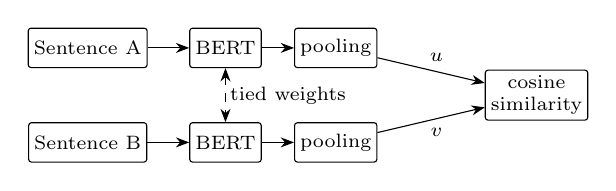
\begin{tikzpicture}[font=\scriptsize, box/.style={draw, rounded corners=1pt, minimum height=5mm, inner sep=2pt, align=center}, >=Stealth]
\node[box] (a) at (0,0.9) {Sentence A};
\node[box] (ba) at (1.75,0.9) {BERT};
\node[box] (pa) at (3.15,0.9) {pooling};
\node[box] (b) at (0,-0.3) {Sentence B};
\node[box] (bb) at (1.75,-0.3) {BERT};
\node[box] (pb) at (3.15,-0.3) {pooling};
\node[box] (c) at (5.7,0.3) {cosine\\similarity};
\draw[->] (a) -- (ba); \draw[->] (ba) -- (pa);
\draw[->] (b) -- (bb); \draw[->] (bb) -- (pb);
\draw[->] (pa) -- node[above, pos=0.55] {$u$} (c);
\draw[->] (pb) -- node[below, pos=0.55] {$v$} (c);
\draw[dashed, <->] (ba) -- node[right, inner sep=1.5pt] {tied weights} (bb);
\end{tikzpicture}
\caption{SBERT at inference: both sentences go through the same network (tied weights), are pooled into fixed-size vectors $u$ and $v$, and are compared with cosine similarity.}
\label{fig:sbert}
\end{figure}

\paragraph{Spearman's correlation by example.}
Spearman's $\rho$ compares rankings, not raw values: $\rho = 1 - 6\sum_i d_i^2 / (n(n^2-1))$, where $d_i$ is the difference between the ranks that the two rankings give to item $i$ (ties receive average ranks). Suppose four sentence pairs have gold scores $4.5, 3.0, 1.0, 2.0$ (ranks $1,2,4,3$) and a model's cosine similarities are $0.91, 0.30, 0.20, 0.80$ (ranks $1,3,4,2$). The rank differences are $0,1,0,-1$, so $\sum_i d_i^2 = 2$ and $\rho = 1 - (6\times 2)/(4\times 15) = 0.8$. The score is insensitive to how cosine values are scaled, which matters in Section~\ref{sec:results}.

\paragraph{Why this paper.}
The choice rests on four criteria. \emph{Venue:} EMNLP is ranked A* in the CORE conference ranking \citep{portalcore}. \emph{Impact:} Semantic Scholar lists more than 11,000 citations \citep{semanticscholar2019sbert}. \emph{Code:} the official \texttt{sentence-transformers} library is actively maintained, with over 17,000 GitHub stars and over 2,600 forks \citep{sentbert_repo}. \emph{Feasibility:} the checkpoints and all datasets are openly downloadable, and the library installed and ran without code changes. I chose it after an earlier candidate, a 2022 log anomaly detection paper, proved infeasible: its 2021 pinned dependencies would not install and I fixed five separate code bugs without getting training to run (Section~\ref{sec:conclusions}).

\section{Datasets Used in the Original Paper}
\label{sec:origdata}

Table~\ref{tab:origdata} lists the datasets the paper uses. In this project I replicated only the STS Benchmark evaluation; the other datasets are listed to show what remains.

\begin{table*}[t]
\centering\small
\begin{tabular}{p{3.0cm}p{4.0cm}p{5.4cm}p{1.5cm}}
\toprule
Dataset & Role in the paper & Size and format & Used here \\
\midrule
SNLI \citep{bowman2015large} & Training & about 570,000 pairs labelled entailment, contradiction or neutral & No \\
MultiNLI \citep{williams2018broad} & Training & about 430,000 pairs, several genres, same labels & No \\
STS 2012--2016 \citep{agirre2012semeval,agirre2016semeval} & Unsupervised STS evaluation & sentence pairs scored 0--5 & No \\
STS Benchmark \citep{cer2017semeval} & STS evaluation and supervised fine-tuning & 8,628 pairs (train 5,749, dev 1,500, test 1,379); captions, news, forums; scored 0--5 & \textbf{Yes} \\
SICK-R \citep{marelli2014sick} & STS evaluation & sentence pairs with relatedness scores 0--5 & No \\
AFS corpus \citep{misra2016afs} & Argument similarity & 6,000 argument pairs on three topics, scored 0--5 & No \\
Wikipedia sections \citep{dor2018wikisections} & Triplet training and evaluation & about 1.8M training and 222,957 test triplets; accuracy & No \\
SentEval \citep{conneau2018senteval} & Transfer classification (MR, CR, SUBJ, MPQA, SST, TREC, MRPC) & logistic regression on embeddings; 10-fold accuracy & No \\
\bottomrule
\end{tabular}
\caption{Datasets used in the original paper (sizes from \citealp{reimers2019sentence}).}
\label{tab:origdata}
\end{table*}

\paragraph{STS Benchmark format.}
Each STSb record is a pair of English sentences with a gold similarity score from 0 (unrelated) to 5 (equivalent). The Hugging Face copy used here has the fields \texttt{sentence1}, \texttt{sentence2} and \texttt{score}, with scores rescaled to 0--1, which does not change Spearman correlation.\footnote{\url{https://huggingface.co/datasets/sentence-transformers/stsb}} A real record from the test split is shown below.

\begin{table}[h]
\centering\small
\begin{tabular}{ll}
\toprule
Field & Value \\
\midrule
\texttt{sentence1} & A girl is styling her hair. \\
\texttt{sentence2} & A girl is brushing her hair. \\
\texttt{score} & 0.5 \\
\bottomrule
\end{tabular}
\caption{One STS Benchmark record (Hugging Face copy).}
\end{table}

\section{Replication of the Original Work}
\label{sec:replication}

All code is in a public GitHub repository.\footnote{\url{https://github.com/hslokapal/comp8240-sbert-reproduction}}

\paragraph{Environment.}
I ran the code in two environments. (1) A Google Colab runtime with Python 3.13, PyTorch 2.11.0, transformers 5.15.1 and sentence-transformers 5.7.0. (2) A MacBook Air (Apple silicon, macOS) in a conda environment with Python 3.10.22, PyTorch 2.14.1, transformers 5.19.0, sentence-transformers 6.1.0, datasets 5.1.0, NumPy 2.2.6, SciPy 1.15.3 and scikit-learn 1.7.2. The scripts write the exact versions to \texttt{results/environment.txt}. The 2019 software stack used by the authors was not recreated, so version differences are a possible source of small deviations.

\paragraph{Procedure.}
For each model the script \texttt{01\_replicate\_stsb.py} (1) loads the 1,379-pair STSb test split, (2) embeds both sentences with the model's own pooling configuration, (3) computes the cosine similarity of each pair, and (4) computes Spearman's $\rho$ against the gold scores, multiplied by 100. I evaluated the two checkpoints released for the paper, \texttt{bert-base-nli-mean-tokens} (the NLI-only base model) and \texttt{bert-base-nli-stsb-mean-tokens} (NLI followed by STSb fine-tuning), plus the later \texttt{all-MiniLM-L6-v2}. The two paper checkpoints are marked as deprecated on the model hub, so they are the closest available match to the paper, not a guarantee of identical weights.

Table~\ref{tab:models} summarises the three models, using details from their Hugging Face model cards.\footnote{\url{https://huggingface.co/sentence-transformers/bert-base-nli-mean-tokens}, \url{https://huggingface.co/sentence-transformers/bert-base-nli-stsb-mean-tokens} and \url{https://huggingface.co/sentence-transformers/all-MiniLM-L6-v2}.}

\begin{table*}[t]
\centering\small\setlength{\tabcolsep}{4pt}
\begin{tabular}{p{3.3cm}p{3.0cm}rrrp{3.8cm}}
\toprule
Model & Base network & Parameters & Dim. & Max input & Training data \\
\midrule
SBERT-NLI-base (paper checkpoint) & BERT-base, mean pooling & 109M & 768 & 128 & SNLI and MultiNLI \\
SBERT-NLI-STSb-base (paper checkpoint) & BERT-base, mean pooling & 109M & 768 & 128 & NLI, then the STSb training split \\
all-MiniLM-L6-v2 (later model) & MiniLM, 6 layers, mean pooling & 22.7M & 384 & 256 & over 1 billion sentence pairs from 21 datasets, including Stack Exchange, WikiAnswers duplicate questions and S2ORC citation pairs \\
\bottomrule
\end{tabular}
\caption{The three models compared. Maximum input is in word pieces.}
\label{tab:models}
\end{table*}

\begin{table}[t]
\centering\small
\begin{tabular}{p{3.6cm}rrr}
\toprule
Model & Paper & Ours & Diff. \\
\midrule
SBERT-NLI-base (paper checkpoint) & 77.03 & 76.98 & $-0.05$ \\
SBERT-NLI-STSb-base (paper checkpoint) & 85.35 & 85.05 & $-0.30$ \\
all-MiniLM-L6-v2 (later model) & -- & 82.03 & -- \\
\bottomrule
\end{tabular}
\caption{Spearman $\rho \times 100$ on the STSb test set (1,379 pairs). Paper values are from \citet{reimers2019sentence}; the STSb-fine-tuned value is a mean over 10 seeds.}
\label{tab:repl}
\end{table}

\paragraph{Results.}
Table~\ref{tab:repl} compares my numbers with the paper's. The result for \texttt{all-MiniLM-L6-v2} was identical on Colab and on my Mac. Both paper checkpoints reproduce the paper's numbers closely: the NLI-only base model scores 76.98 against the paper's 77.03 ($-0.05$), and the model with STSb fine-tuning scores 85.05 against 85.35 ($-0.30$). The second gap is slightly larger than the $\pm 0.17$ the paper reports across seeds; I attribute it to comparing one released checkpoint with a mean over 10 seeds, though I did not test this. That \texttt{all-MiniLM-L6-v2} scores higher than the paper's NLI-only 77.03 is expected and is not a replication of the paper's number: it is a later model trained on a much larger and more varied set of sentence pairs. I therefore treat it as evidence that the evaluation pipeline works, not as a reproduction of the paper's result.

\paragraph{Reasons results might differ.}
Possible reasons for any gap are: (i) the hosted checkpoints are re-uploads from 2020 and may not be bit-identical to the paper's models; (ii) the paper's supervised numbers are means over 10 random seeds, whereas a released checkpoint is one run; (iii) different library versions change tokenisation and numerical details; (iv) the checkpoints truncate input at 128 tokens; and (v) the Hugging Face STSb copy rescales scores, though this cannot change a rank correlation.

\section{Construction of New Data}
\label{sec:newdata}

\subsection{An Existing Dataset: BIOSSES}
BIOSSES \citep{soganciouglu2017biosses} contains 100 biomedical sentence pairs taken from citing sentences in articles of the TAC Biomedical Summarization track. Each pair was scored from 0 (no relation) to 4 (equivalent) by five human experts, and the dataset gives the mean. It is released under GPL-3.0 and I load it from the Hugging Face Hub without copying it into my repository.\footnote{\url{https://huggingface.co/datasets/tabilab/biosses}} No preprocessing is needed, because Spearman correlation is unaffected by the 0--4 scale. I chose it because its specialised vocabulary makes it the nearest available test of whether SBERT carries over to technical text. My proposal also listed Quora Question Pairs, PAWS and Stack Exchange duplicates; I did not run them for lack of time, which limits how widely I can claim generalisation.

\subsection{A Constructed Dataset: Data-Engineering Questions}
\paragraph{Design.}
I constructed 40 sentence pairs in my own professional domain: Azure Data Factory, Databricks, PySpark, Synapse and the medallion architecture. The pairs fall into four bands: 13 near-paraphrases (high similarity), 12 same-topic pairs asking different things (medium), 13 pairs from the same domain but unrelated questions (low), and 2 anchor pairs on unrelated topics. Table~\ref{tab:snippet} shows real rows from the data.

\paragraph{How the pairs were produced.}
The sentences were drafted with the help of a large language model (Claude), in the style of real data-engineering questions; they are not copied from documentation or forums, which also avoids reusing text under third-party licences. The model also suggested an initial score for each pair. I read all 40 pairs and revised three scores after deciding the model had over-rated or under-rated them: pair 14 (scheduling versus monitoring a pipeline, 2.3 to 1.6), pair 20 (schema drift versus a tumbling-window trigger, 1.5 to 0.6, which moved it from the medium to the low band) and pair 26 (a notebook running out of memory versus converting a Pandas DataFrame, 1.4 to 2.0). The pairs were then stored in the STS format (CSV with a pair ID, two sentences and a score) and a shuffled copy with blank scores was made for the other raters. Sentences were left as written, with no cleaning. The data and scripts are in the repository.

\paragraph{Why these bands.}
The bands were fixed before scoring so the set covers the whole similarity range. Near-paraphrases test whether a model recognises the same question in different words. Same-topic pairs that ask for different things test whether it separates topic from task. Low pairs share only the broad domain, and the two anchors give the scale a floor. The 40 pairs use 53 distinct sentences, and 13 of those appear in two to four pairs, so one question is compared with paraphrased, related and unrelated partners.

\begin{table*}[t]
\centering\small
\begin{tabular}{rp{5.6cm}p{5.6cm}rl}
\toprule
ID & Sentence 1 & Sentence 2 & A1 & Band \\
\midrule
1 & How do I schedule a pipeline to run every night in Azure Data Factory? & What's the best way to set up a daily trigger for an ADF pipeline? & 4.8 & high \\
7 & Why is my Spark job spilling to disk during a shuffle? & What causes disk spill during a shuffle stage in a Spark job? & 4.8 & high \\
17 & What does the bronze layer store in a medallion architecture? & What transformations typically happen in the silver layer of a medallion architecture? & 2.8 & medium \\
14 & How do I schedule a pipeline to run every night in Azure Data Factory? & How do I monitor pipeline failures in Azure Data Factory? & 1.6 & medium \\
20 & How do I handle schema drift in an ADF copy activity? & How do I set up a tumbling window trigger in ADF? & 0.6 & low \\
39 & How do I schedule a pipeline to run every night in Azure Data Factory? & What's a good recipe for pasta carbonara? & 0.0 & anchor \\
\bottomrule
\end{tabular}
\caption{Rows from the constructed dataset (A1 = annotator 1's score on the 0--5 scale).}
\label{tab:snippet}
\end{table*}

\subsection{Annotation and Agreement}
\paragraph{Raters.}
\emph{Annotator 1} is me. Because my scores began as LLM suggestions, they are not fully independent of the LLM. \emph{Annotator 2} is 
a friend with data engineering experience, who volunteered, was given the written guidelines and used no AI tools; they scored the shuffled blank sheet alone, without seeing my scores. The \emph{LLM judge} is Gemini (Google), a different model family from the one that drafted the pairs. It was used through a Google AI Pro subscription in a new chat on 9 November 2026 and given only the blank sheet; I did not record the exact model version shown in the app. Annotators used the 0--5 scale adapted from the SemEval STS guidelines (Appendix~\ref{sec:appendix}).

\paragraph{Agreement.}
I report Spearman's $\rho$ and quadratic-weighted Cohen's $\kappa$ on scores rounded to integers 0--5, which suits an ordinal scale. Annotator 1 versus annotator 2: $\rho=0.95$, $\kappa=0.95$, mean absolute difference 0.4 points; the two scores are within one point on 97.5\% of pairs and agree exactly after rounding on 60\%. Only two pairs differ by a point or more (pairs 15 and 17, both same-topic pairs that ask for different things), and annotator 2 scored the medium band lower on average (1.38 against my 2.10), so annotator 2 was stricter about pairs that share a tool or topic but ask for different things. This high agreement is partly an effect of the design: the bands were chosen to be easy to separate, so it should not be read as agreement on difficult natural data. The LLM judge versus annotator 1: $\rho=0.95$, $\kappa=0.95$; versus annotator 2: $\rho=0.97$, $\kappa=0.99$. The judge graded coarsely, using only the values 0, 1, 2 and 5, and gave all 13 near-paraphrases 5.0 where the humans gave 4.5 to 4.9. On the 12 medium pairs both annotator 2 and the LLM were stricter than I was (means 1.38 and 1.25 against my 2.10), so my scores are the outlier in that band.

\begin{table}[t]
\centering\small
\begin{tabular}{lcccc}
\toprule
Band & $n$ & A1 & A2 & LLM \\
\midrule
High & 13 & 4.78 & 4.91 & 5.00 \\
Medium & 12 & 2.10 & 1.38 & 1.25 \\
Low & 13 & 0.50 & 0.18 & 0.08 \\
Anchor & 2 & 0.00 & 0.00 & 0.00 \\
All & 40 & 2.34 & 2.07 & 2.02 \\
\bottomrule
\end{tabular}
\caption{Mean score by band for annotator 1 (A1), annotator 2 (A2) and the LLM judge. The raters differ mainly in the medium band.}
\label{tab:bands}
\end{table}

\paragraph{Quality compared with the original data.}
The constructed set is far smaller than STSb (40 pairs against 8,628) and has two human raters plus one LLM, where BIOSSES used five experts. Its bands were chosen deliberately, so it is not a natural sample of questions. It is suitable for a small, indicative test, not for a published benchmark.

\section{Results on New Data}
\label{sec:results}

Table~\ref{tab:results} gives Spearman's $\rho \times 100$ for each model on each dataset. Confidence intervals are 95\% bootstrap intervals computed by the scripts.

\begin{table*}[t]
\centering\small
\begin{tabular}{lcccc}
\toprule
Model & STSb test & BIOSSES & Constructed vs A1 & Constructed vs A2 \\
 & ($n$=1379) & ($n$=100) & ($n$=40) & ($n$=40) \\
\midrule
SBERT-NLI-base (paper checkpoint) & 76.98 & \shortstack{51.99\\{\scriptsize CI 35.4--65.6}} & \shortstack{58.89\\{\scriptsize CI 33.3--76.4}} & 57.08 \\
all-MiniLM-L6-v2 (later model) & 82.03 & \shortstack{81.25\\{\scriptsize CI 71.7--88.1}} & \shortstack{83.78\\{\scriptsize CI 72.0--89.3}} & 85.91 \\
\bottomrule
\end{tabular}
\caption{Spearman $\rho \times 100$ between cosine similarity and human scores.}
\label{tab:results}
\end{table*}

\paragraph{How the new results relate to the replication.}
On the constructed data the later model's correlation with annotator 1 (83.78) is close to its STSb score (82.03), which suggests SBERT-style embeddings rank technical questions about as well as general sentences. This comparison is not like for like, for three reasons. First, with $n=40$ the 95\% bootstrap interval for the later model is wide (72.0 to 89.3), so a gap of 1.7 points means nothing. Second, I spread the pairs deliberately from near-paraphrases to unrelated topics, and ranking such a spread is easier than ranking the narrower range in a natural sample. Third, annotator 1's scores began as LLM suggestions. Where the new evaluation differs from the replication, the replication (STSb) is the more trustworthy number. The paper's own checkpoint does much worse on the constructed data (58.89, interval 33.3 to 76.4) than on STSb (76.98) and well below the later model (83.78), although the two intervals overlap slightly. A possible reason is that the NLI-only checkpoint was trained only on inference sentence pairs, whereas the later model's training mix includes Stack Exchange question--answer pairs and duplicate-question collections (Table~\ref{tab:models}), which resemble my constructed questions; I did not test this, and I did not check for overlap between its training data and my sentences. The same pattern holds on BIOSSES: the paper's checkpoint scores 51.99 (interval 35.4 to 65.6) against 81.25 (71.7 to 88.1) for the later model. Its training mix also includes S2ORC scientific citation pairs, which may help on BIOSSES, itself built from citing sentences; this is also untested. Relative to STSb, the NLI-only checkpoint therefore loses 18 points on the constructed data and 25 on BIOSSES, while the later model stays within 2.6 points of its STSb score on both.

\begin{figure}[t]
\centering
\IfFileExists{constructed_scatter.pdf}{\includegraphics[width=0.85\columnwidth]{constructed_scatter.pdf}}{\fillme{copy results/constructed\_scatter.pdf from the repository into this folder}}
\caption{Cosine similarity of all-MiniLM-L6-v2 against annotator 1's score for the 40 constructed pairs.}
\label{fig:scatter}
\end{figure}

\paragraph{Where the model and the humans disagree.}
Figure~\ref{fig:scatter} plots the model's cosine similarity against my scores. The clearest disagreement is pair 14: I scored it 1.6, but the model's cosine similarity is about 0.68, high for a pair that asks about scheduling in one sentence and monitoring in the other. Both sentences share the terms ``pipeline'' and ``Azure Data Factory'', which suggests the model leans on shared vocabulary. The eight largest rank gaps (script 02; Table~\ref{tab:gaps}) include clear errors in both directions. It over-rates pairs that share vocabulary but ask different things: pair 14 (cosine 0.68 against my 1.6) and pair 34, a Databricks cluster question against a PySpark \texttt{explode} question (cosine 0.29 against my 0.3). It under-rates pairs that are related or equivalent in meaning but use different words: pair 22, incremental loading against using a watermark column (cosine 0.13 against my 2.9, since a watermark is the standard technique), and pair 1, a near-paraphrase of a scheduling question (cosine 0.49 against my 4.8, with ``every night'' against ``daily trigger''). Both errors are consistent with the model relying heavily on surface vocabulary. The other four large gaps (pairs 13, 4, 30 and 38) are ordering differences inside a band in which all three raters give nearly the same score, so they say little. I first compared values by rescaling cosine to 0--5, which made unrelated pairs look as if the model rated them about 2.6. Their raw cosine is about 0.05, essentially zero, so the model handles them correctly and the gap came from my rescaling. I now compare ranks, which do not depend on any rescaling.

\begin{table*}[t]
\centering\footnotesize\setlength{\tabcolsep}{3pt}
\begin{tabular}{rp{5.0cm}p{5.0cm}rrrr}
\toprule
ID & Sentence 1 & Sentence 2 & A1 & A2 & LLM & Cosine \\
\midrule
22 & How do I set up incremental loading in Azure Data Factory? & How do I use a watermark column to track changed rows? & 2.9 & 2.3 & 2.0 & 0.13 \\
34 & Why does my Databricks cluster keep auto-terminating? & How do I use the explode function in PySpark? & 0.3 & 0.2 & 0.0 & 0.29 \\
14 & How do I schedule a pipeline to run every night in Azure Data Factory? & How do I monitor pipeline failures in Azure Data Factory? & 1.6 & 1.0 & 1.0 & 0.68 \\
30 & Why is my Spark job spilling to disk during a shuffle? & What's the difference between a managed table and an external table? & 0.8 & 0.5 & 0.0 & 0.01 \\
1 & How do I schedule a pipeline to run every night in Azure Data Factory? & What's the best way to set up a daily trigger for an ADF pipeline? & 4.8 & 4.5 & 5.0 & 0.49 \\
13 & How do I enable autoscaling for a Databricks cluster? & What's the setting to turn on autoscaling in Databricks? & 4.6 & 4.5 & 5.0 & 0.91 \\
38 & What's the best partitioning strategy for a PySpark DataFrame before writing to Delta Lake? & How do I configure a self-hosted integration runtime for on-premises data? & 0.3 & 0.0 & 0.0 & 0.14 \\
4 & How can I optimize a PySpark join between two large DataFrames? & What's the fastest way to join two big PySpark DataFrames? & 4.7 & 5.0 & 5.0 & 0.92 \\
\bottomrule
\end{tabular}
\caption{The eight pairs with the largest rank gap between all-MiniLM-L6-v2 and annotator 1 (output of script 02), with all three raters' scores and the model's cosine similarity.}
\label{tab:gaps}
\end{table*}

\paragraph{How the LLM judge fitted in.}
The proposal planned to use an LLM to explain only the pairs where SBERT disagreed most with the humans. I simplified this: the LLM judge scored all 40 pairs blind, so it acts as a third rater whose scores can be set against the humans' and against SBERT's. This helps separate two explanations for a large model-versus-human gap: the pair is ambiguous (the LLM and the humans also disagree) or the model is wrong (the humans and the LLM agree with each other). The data support model error over annotation ambiguity for the model's largest gaps. On the eight pairs where the model disagrees most with me, annotator 2 and the LLM judge both score within one point of my score (for example pair 14: 1.6, 1.0 and 1.0 against a cosine of 0.68; pair 1: 4.8, 4.5 and 5.0 against 0.49), so the raters agree with each other and the model is the odd one out. The pairs where the raters differ most are different ones (pairs 21, 15, 26, 23 and 22): medium pairs that ask about different tasks in the same tool, where I scored about 2 and the LLM scored 1 (2 for pair 22), and these are where my own scores are least reliable. SBERT's cosine ranks pairs closer to the LLM judge ($\rho=0.89$) than to my scores ($\rho=0.84$), which fits my scores being the most generous in the medium band. Limits: the judge was run once with one prompt, LLM output can vary between runs, and it may share biases with the model that drafted the pairs.

\paragraph{Threats to validity.}
Several limits qualify these results. \emph{Size and dependence:} 40 pairs is small, and the pairs are not independent, because 13 of the 53 distinct sentences appear in more than one pair; the bootstrap intervals resample pairs, so they are probably too narrow. \emph{Provenance:} LLM-drafted questions are probably cleaner and more regular than real ones, so scores may overstate performance on real questions, and the drafting model and the judge may share biases even though they come from different families. \emph{Rater independence:} annotator 1 began from LLM suggestions, whereas annotator 2 and the judge scored blind. \emph{Training-data familiarity:} the later model's training mix includes technical question--answer text, so its strength here may reflect familiarity and not general ability. \emph{Coverage:} I tested two model families, one released checkpoint each, on three datasets. \emph{Metric:} Spearman correlation ignores the absolute scale of cosine scores, which matters if a fixed threshold is used in practice.

\section{Code and Data Availability}
\label{sec:code}

Everything needed to rerun the results is in the repository linked in Section~\ref{sec:replication}. The folder \texttt{scripts/} holds four numbered scripts that run in order: the STSb replication, the constructed-data evaluation, the BIOSSES evaluation and the agreement analysis. The folder \texttt{data/} holds the 40 constructed pairs, the blank annotation sheet and the scores from the second annotator and the LLM judge, and \texttt{results/} holds the saved outputs (environment, per-pair scores and agreement statistics). The README gives setup commands for Python 3.10, with the package versions pinned in \texttt{requirements.txt}. The first three scripts download models and datasets on first use and each ran in a few minutes on a laptop CPU; the fourth needs no internet. The STS Benchmark and BIOSSES are not copied into the repository.

\section{Ethical Considerations}
\label{sec:ethics}

I use the eight principles of the Australian Code for the Responsible Conduct of Research \citep{nhmrc2018code}: honesty, rigour, transparency, fairness, respect, recognition, accountability and promotion of responsible research practices. The unit's ethics page also points to two documents that bear on this project. The National Statement on Ethical Conduct in Human Research \citep{nhmrc2025national} covers research involving people, and the University's Responsible and Ethical Use of Artificial Intelligence Policy \citep{mqai2025policy} applies to students as well as staff. I take the first as a reason to check ethics requirements before publishing, as set out below, and the second as a reason to disclose and take responsibility for the AI assistance in this project.

\paragraph{Issues in the original paper.}
\emph{Bias and fairness.} SBERT is built on BERT, pretrained on Wikipedia and books, and trained on crowd-sourced NLI data. Sentence encoders can encode social biases, which \citet{may2019measuring} set out to measure, and the paper reports no bias evaluation of SBERT. Embeddings used for search or clustering could therefore treat groups unequally. \emph{Rigour and transparency.} The authors use multiple random seeds for supervised results and release code and models, which supports reproducibility. The unsupervised results in Table 1 of the paper are single numbers without confidence intervals. \emph{Privacy.} Embedding personal text for semantic search can make private information easier to retrieve, a risk the paper does not discuss. \emph{Open access.} The paper is on arXiv and the ACL Anthology and the checkpoints are Apache-2.0 licensed according to their model cards, which supports open access and verification. The deprecated status of the checkpoints shows that released artefacts can lose support over time.

\paragraph{If I published a paper on the new data.}
\emph{Honesty and transparency.} I would state that the sentences were drafted with LLM assistance and that annotator 1's scores began as LLM suggestions, report the agreement statistics and the small sample size, and not present the constructed set as a natural benchmark. \emph{Rigour.} I would add more pairs, collect them from real documentation or Q\&A text by script, use more than two annotators, and fix the annotation protocol before scoring. \emph{Fairness, respect and recognition.} Annotator 2 is a human participant: taking part was voluntary, no personal data was collected, and when I asked after scoring, they agreed that their 40 scores, labelled only as annotator 2, could be published in the appendix and the repository. For publication I would check whether institutional ethics review applies and I would acknowledge the annotator. The Code's principle on the rights of Aboriginal and Torres Strait Islander peoples is not directly engaged, because the data concern software questions and involve no community. \emph{Accountability and data licensing.} I am responsible for all content, including AI-assisted parts. BIOSSES is GPL-3.0 and STSb is a third-party resource, so I load them from their hosts and do not redistribute them. The constructed data contains no personal information. I release it under the Creative Commons Attribution 4.0 licence (CC BY 4.0), and the code under the MIT licence.

\section{Conclusions and Reflections}
\label{sec:conclusions}

\paragraph{How far the replication went.}
The evaluation pipeline reproduces expected behaviour: the later model scores 82.03 on STSb, identically in two environments. The paper's own checkpoints reproduce its STSb numbers to within 0.3 points (76.98 against 77.03, and 85.05 against 85.35). I did not replicate the STS 2012--2016, SICK-R, argument-similarity, Wikipedia-sections or SentEval results, I did not retrain any model, and I did not test the paper's efficiency claim (about 5 seconds to embed 10,000 sentences).

\paragraph{How well the approach generalised.}
On BIOSSES and the constructed data the later model held up (81.25 and 83.78, against 82.03 on STSb) while the paper's own NLI-only checkpoint fell sharply (51.99 and 58.89, against 76.98). The evidence from the constructed set is weak for the reasons given in Section~\ref{sec:results}, so I would call generalisation to technical text plausible but not established.

\paragraph{Reflections.}
(1) A better way to build the dataset would have been to collect real questions by script from documentation or Q\&A sites and have several people score them from the start, instead of drafting pairs with an LLM and reviewing its scores. (2) Annotation was harder than expected for pairs that share vocabulary but ask different things; the three scores I revised were all of this kind. (3) Comparing rescaled cosine values misled me; rank-based comparison is safer. (4) The first candidate paper taught me to check feasibility early: its 2021 pinned dependencies would not install, and I fixed five code bugs (a sample-size type error, a mismatched output folder, a column-count mismatch, a missing \texttt{Seq} key and a missing embeddings file) before training still failed on the first batch. Switching to a maintained library cost less than continuing.

\begingroup
\makeatletter
\expandafter\def\expandafter\UrlBreaks\expandafter{\UrlBreaks\do\0\do\1\do\2\do\3\do\4\do\5\do\6\do\7\do\8\do\9}
\makeatother
\bibliography{custom}
\endgroup

\appendix
\section{Annotation Scale and LLM-Judge Prompt}
\label{sec:appendix}
The 0--5 scale adapted from the SemEval STS guidelines: 5 completely equivalent; 4 mostly equivalent, unimportant details differ; 3 roughly equivalent, some important information differs; 2 not equivalent but share some details; 1 not equivalent but on the same topic; 0 completely dissimilar. Annotators were told to judge meaning, not shared words. The LLM judge received the same scale, the instruction to output only a CSV of \texttt{pair\_id,score}, and the 40 blank pairs in shuffled order. The exact prompt is in \texttt{docs/annotation\_guidelines.md} in the repository.


\section{The Constructed Dataset}
\label{sec:appendixdata}
Tables~\ref{tab:data1} and~\ref{tab:data2} list all 40 pairs with the scores from annotator 1 (A1), annotator 2 (A2) and the LLM judge. IDs 1--13 are the high band, 14--26 the medium band (except 20, which is low), 27--38 the low band and 39--40 the anchors.

\begin{table*}[t]
\centering\scriptsize\setlength{\tabcolsep}{3pt}
\begin{tabular}{rp{6.3cm}p{6.3cm}rrr}
\toprule
ID & Sentence 1 & Sentence 2 & A1 & A2 & LLM \\
\midrule
1 & How do I schedule a pipeline to run every night in Azure Data Factory? & What's the best way to set up a daily trigger for an ADF pipeline? & 4.8 & 4.5 & 5.0 \\
2 & My Databricks notebook keeps running out of memory when processing a large CSV. & I'm getting out-of-memory errors in a Databricks notebook while reading a big CSV file. & 4.9 & 5.0 & 5.0 \\
3 & What is the difference between a mapping data flow and a wrangling data flow in ADF? & How do mapping data flows differ from wrangling data flows in Azure Data Factory? & 4.9 & 5.0 & 5.0 \\
4 & How can I optimize a PySpark join between two large DataFrames? & What's the fastest way to join two big PySpark DataFrames? & 4.7 & 5.0 & 5.0 \\
5 & What does the bronze layer store in a medallion architecture? & In a medallion architecture, what kind of data lives in the bronze layer? & 4.9 & 5.0 & 5.0 \\
6 & How do I parameterize a linked service in Azure Data Factory? & What's the process for making an ADF linked service accept parameters? & 4.6 & 5.0 & 5.0 \\
7 & Why is my Spark job spilling to disk during a shuffle? & What causes disk spill during a shuffle stage in a Spark job? & 4.8 & 5.0 & 5.0 \\
8 & How do I connect Synapse Analytics to a Power BI dashboard? & What steps are needed to link Azure Synapse to Power BI? & 4.7 & 4.8 & 5.0 \\
9 & How do I handle schema drift in an ADF copy activity? & What's the recommended way to deal with schema drift when copying data in ADF? & 4.8 & 5.0 & 5.0 \\
10 & What's the best partitioning strategy for a PySpark DataFrame before writing to Delta Lake? & How should I partition a PySpark DataFrame before saving it as a Delta table? & 4.9 & 5.0 & 5.0 \\
11 & How do I set up incremental loading in Azure Data Factory? & What's the standard approach for incremental data loads in ADF? & 4.7 & 5.0 & 5.0 \\
12 & Why does my Databricks cluster keep auto-terminating? & What causes a Databricks cluster to shut down automatically? & 4.8 & 5.0 & 5.0 \\
13 & How do I enable autoscaling for a Databricks cluster? & What's the setting to turn on autoscaling in Databricks? & 4.6 & 4.5 & 5.0 \\
14 & How do I schedule a pipeline to run every night in Azure Data Factory? & How do I monitor pipeline failures in Azure Data Factory? & 1.6 & 1.0 & 1.0 \\
15 & What is the difference between a mapping data flow and a wrangling data flow in ADF? & How do I debug a data flow in Azure Data Factory? & 2.2 & 1.0 & 1.0 \\
16 & How can I optimize a PySpark join between two large DataFrames? & How do I read a Parquet file into a PySpark DataFrame? & 1.8 & 1.0 & 1.0 \\
17 & What does the bronze layer store in a medallion architecture? & What transformations typically happen in the silver layer of a medallion architecture? & 2.8 & 1.8 & 2.0 \\
18 & Why is my Spark job spilling to disk during a shuffle? & How do I increase the number of shuffle partitions in Spark? & 2.6 & 2.2 & 2.0 \\
19 & How do I connect Synapse Analytics to a Power BI dashboard? & How do I create a serverless SQL pool in Azure Synapse? & 1.7 & 1.0 & 1.0 \\
20 & How do I handle schema drift in an ADF copy activity? & How do I set up a tumbling window trigger in ADF? & 0.6 & 1.0 & 1.0 \\
\bottomrule
\end{tabular}
\caption{Constructed dataset, pairs 1--20, with the three raters' scores.}
\label{tab:data1}
\end{table*}
\begin{table*}[t]
\centering\scriptsize\setlength{\tabcolsep}{3pt}
\begin{tabular}{rp{6.3cm}p{6.3cm}rrr}
\toprule
ID & Sentence 1 & Sentence 2 & A1 & A2 & LLM \\
\midrule
21 & What's the best partitioning strategy for a PySpark DataFrame before writing to Delta Lake? & How do I perform an upsert into a Delta table? & 2.4 & 1.8 & 1.0 \\
22 & How do I set up incremental loading in Azure Data Factory? & How do I use a watermark column to track changed rows? & 2.9 & 2.3 & 2.0 \\
23 & Why does my Databricks cluster keep auto-terminating? & How do I attach a notebook to an existing Databricks cluster? & 1.9 & 1.0 & 1.0 \\
24 & How do I parameterize a linked service in Azure Data Factory? & How do I create a self-hosted integration runtime in ADF? & 1.6 & 1.0 & 1.0 \\
25 & How do I enable autoscaling for a Databricks cluster? & How do I install a Python library on a Databricks cluster? & 1.7 & 1.0 & 1.0 \\
26 & My Databricks notebook keeps running out of memory when processing a large CSV. & How do I convert a Pandas DataFrame to a PySpark DataFrame? & 2.0 & 1.5 & 1.0 \\
27 & How do I schedule a pipeline to run every night in Azure Data Factory? & What's the syntax for a PySpark window function? & 0.6 & 0.0 & 0.0 \\
28 & What does the bronze layer store in a medallion architecture? & How do I reset my Databricks workspace password? & 0.3 & 0.2 & 0.0 \\
29 & How can I optimize a PySpark join between two large DataFrames? & How do I create a Synapse workspace from the Azure portal? & 0.5 & 0.0 & 0.0 \\
30 & Why is my Spark job spilling to disk during a shuffle? & What's the difference between a managed table and an external table? & 0.8 & 0.5 & 0.0 \\
31 & How do I connect Synapse Analytics to a Power BI dashboard? & How do I write unit tests for a PySpark transformation function? & 0.4 & 0.0 & 0.0 \\
32 & How do I handle schema drift in an ADF copy activity? & What is the purpose of a checkpoint in Spark Structured Streaming? & 0.7 & 0.3 & 0.0 \\
33 & How do I set up incremental loading in Azure Data Factory? & How do I enable row-level security in Synapse? & 0.5 & 0.1 & 0.0 \\
34 & Why does my Databricks cluster keep auto-terminating? & How do I use the explode function in PySpark? & 0.3 & 0.2 & 0.0 \\
35 & How do I parameterize a linked service in Azure Data Factory? & What's the difference between RDD and DataFrame in Spark? & 0.6 & 0.0 & 0.0 \\
36 & How do I enable autoscaling for a Databricks cluster? & How do I create a stored procedure in Synapse SQL pool? & 0.4 & 0.0 & 0.0 \\
37 & My Databricks notebook keeps running out of memory when processing a large CSV. & How do I set up CI/CD for an ADF pipeline using Azure DevOps? & 0.5 & 0.1 & 0.0 \\
38 & What's the best partitioning strategy for a PySpark DataFrame before writing to Delta Lake? & How do I configure a self-hosted integration runtime for on-premises data? & 0.3 & 0.0 & 0.0 \\
39 & How do I schedule a pipeline to run every night in Azure Data Factory? & What's a good recipe for pasta carbonara? & 0.0 & 0.0 & 0.0 \\
40 & What does the bronze layer store in a medallion architecture? & What time does the next train leave the station? & 0.0 & 0.0 & 0.0 \\
\bottomrule
\end{tabular}
\caption{Constructed dataset, pairs 21--40, with the three raters' scores.}
\label{tab:data2}
\end{table*}

\end{document}
